\documentclass[a4paper,utf8]{article}
\usepackage[heading,fancyhdr]{ctex}
\usepackage{amsmath,amssymb,geometry,lastpage,ulem}
\usepackage{array,tabularx,tabulary,mhchem,xspace}
\usepackage{floatrow,subfig,multirow,bigstrut}
\usepackage{siunitx,booktabs,longtable,graphicx,xfrac,nameref}
\lineskiplimit=1pt
\lineskip=3pt
\geometry{
    top=25.4mm, 
    left=25mm, 
    right=25mm, 
    bottom=25mm,
    headsep=5.9mm,
}
\ctexset{
    section = {format+=\raggedright}
}
\newcommand{\fgref}[1]{图~\ref{#1}\xspace}
\newcommand{\seqref}[1]{式~(\ref{#1})}
\newcommand{\expinfo}[7][无]{
    {\zihao{-3}\bfseries\songti
    实验名称:\uline{\hfill\mbox{#2}\hfill} \\[2.9mm]
    学\quad 号:\uline{\makebox[25mm]{#3}}\hfill
    姓\quad 名:\uline{\makebox[25mm]{#4}}\hfill
    班\quad 级:\uline{\makebox[25mm]{#5}} \\[2.9mm]
    合作者:\uline{\makebox[25mm]{#1}} \hfill
    桌\quad 号:\uline{\makebox[25mm]{#6}}\hfill\makebox[25mm+4em]{}\\[2.9mm]
    实验日期:\uline{\makebox[30mm]{#7}}\hfill\mbox{} \\[58.7mm]
    }
}
\newcommand{\pointingbox}{
    {\zihao{4}\bfseries\songti%
    实验考核\\[3mm]
    \extrarowheight=3mm
    \begin{tabularx}{150mm}{|X|X|X|X|X|}\hline
        \hfil 项目 \hfil  & \hfil 实验预习 \hfil & \hfil 实验过程 \hfil & \hfil 分析与讨论 \hfil & \hfil 总评 \hfil \\[3mm] \hline
        \hfil 评价 \hfil &  &  &  &  \\[3mm] \hline
    \end{tabularx}
    }
}
\newcommand{\derivative}[2]{\frac{\mathrm{d} #1}{\mathrm{d} #2}}
\newcommand{\thinking}[2]{\textbf{#1}\\
答:\begin{minipage}[t]{0.85\textwidth}
    #2
\end{minipage}}
\pagestyle{fancy}
\fancyhf{} \fancyhead[C]{电路基础实验} \fancyfoot[C]{\thepage~/~\pageref{LastPage}}
\newcounter{Rownumber}
\newcommand*{\Rown}{\stepcounter{Rownumber}\theRownumber}
\newcommand*{\resetRown}{\setcounter{Rownumber}{0}}
\newcommand{\qrange}[3]{\qtyrange[range-phrase = \text{$\sim$},range-units =single]{#1}{#2}{#3}}
\floatsetup[table]{capposition=top}
\newcolumntype{C}{>{\hfil}X<{\hfil}}
\renewcommand{\Nameref}[1]{\textbf{\ref{#1}~\nameref{#1}}} %导入导言

\begin{document}
\begin{center}
    {\mbox{}\\[7em]\zihao{2}\bfseries\songti%
    电路基础实验报告}\\[34mm]
    \expinfo[张泽钒]{戴维南定理和诺顿定理}{22301077}{张蕴东}{22高分子}{35}{2024.5.21}
\end{center}
\newpage
\section{实验目的}
\begin{enumerate}
    \item 加深对戴维南定理和诺顿定理的理解。
    \item 学习戴维南等效参数的各种测量方法。
    \item 理解等效置换的概念。
    \item 学习直流稳压电源、万用表、直流电流表和电压表的正确使用方法。
\end{enumerate}

\section{实验原理}%简单描述,含必要的公式和附图;
\subsection{戴维南定理}
戴维南定理是指一个含独立电源、线性电阻和受控源的一端口,对外电路来说,可以用一个电压源和一个电阻的串联组合来等效置换。此电压源的电压等于该端口的开路电压 $U_\text{OC}$,而电阻等于该端口的全部独立电源置零后的输入电阻,如图~\ref{fig:a} 所示。这个电压源和电阻的串联组合称为戴维南等效电路。等效电路中的电阻称为戴维南等效电阻 $R_\text{eq}$。\par
所谓等效是指用戴维南等效电路把有源一端口网络置换后,对有源端口(1-1’)以外的电路的求解是没有任何影响的,也就是说对端口 1-1’以外的电路而言,电流和电压仍然等于置换前的值。外电路可以是不同的。
\subsection{诺顿定理}
诺顿定理是戴维南定理的对偶形式,它指出一个含独立电源、线性电阻和受控源的一端口,对外电路来说,可以用一个电流源和电导的并联组合来等效置换,电流源的电流等于该一端口的短路电流 $I_\text{SC}$,而电导等于把该一端口的全部独立电源置零后的输入电导 $G_\text{eq}=\frac{1}{R_\text{eq}}$,见图~\ref{fig:a}。\par
戴维南—诺顿定理的等效电路是对外部特性而言的,也就是说不管是时变的还是定常的,只要含源网络内部除独立的电源外都是线性元件,上述等值电路都是正确的。
\begin{figure}[!ht]
    \caption{一端口网络的等效置换\label{fig:a}}
    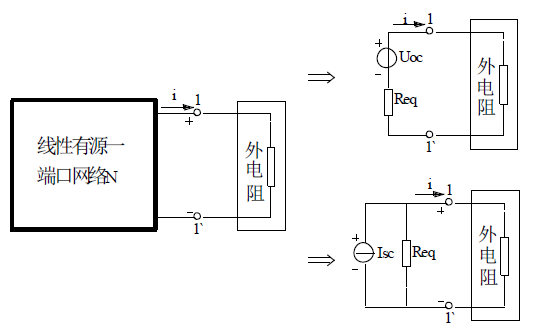
\includegraphics[width=0.6\textwidth]{1.png}
\end{figure}

\section{实验仪表}
    RIGOL DM3058 万用表、RIGOL DP832 直流稳压电源、电路分析实验箱、导线若干。
\section{实验内容}
\begin{enumerate}
    \item 计算与测量有源一端口网络的开路电压、短路电流
    \begin{enumerate}
        \item 计算有源一端口网络的开路电压 $U_\text{OC}$、短路电流 $I_\text{SC}$。结果记入表~\ref{tab:1} 中。
        \item 测量有源一端口网络的开路电压 $U_\text{OC}$,可采用以下几种方法:
        \begin{enumerate}
            \item 直接测量法。
            \item 间接测量法。又称补偿法,分为补偿法一、补偿法二、补偿法三。
        \end{enumerate}
    \end{enumerate}
    \item 计算与测量有源一端口网络的等效电阻 $R_\text{eq}$
    \begin{enumerate}
        \item 计算有源一端口网络的等效电阻 $R_\text{eq}$。当一端口网络内部无源时(把双刀双投开关 K1 合向短路线),计算有源一端口网络的等效电阻 $R_\text{eq}$。把计算结果记入表~\ref{tab:1} 中。
        \item 测量有源一端口网络的等效电阻 $R_\text{eq}$。可根据一端口网络内部是否有源,分别采用如下方法测量:
        \begin{enumerate}
            \item 开路电压、短路电流法。
            \item 伏安法。
            \item 半流法。
            \item 半压法。
            \item 直接测量法。
        \end{enumerate}
    \end{enumerate}
    \item 验证戴维南定理,理解等效概念
    \item 验证诺顿定理,理解等效概念
\end{enumerate}

\section{实验结果与分析}
    \subsection{实验结果}
        实验结果如表~1-5 所示。
        \begin{table}[!ht]\caption{戴维南等效参数计算}
            \begin{tabularx}{0.55\textwidth}{CC} \toprule
                参数 & 计算值 \\ \midrule
                $U_\text{OC}$ & \SI{4}{\V} \\
                $I_\text{SC}$ & \SI{20}{\mA} \\
                $R_\text{eq}$ & \SI{200}{\ohm} \\ \bottomrule
            \end{tabularx}
        \end{table}
        \newpage
        \begin{table}[!ht]\caption{等效电压源电压 $U_\text{OC}$ 测量结果}
            \begin{tabularx}{0.55\textwidth}{CC} \toprule
                方法 & $U_\text{OC}$(\unit{\V}) \\ \midrule
                直接测量 & 3.97 \\
                补偿法之一 & $2.5 \sim 5.6$ \\
                补偿法之二 & 4.074 \\
                补偿法之三 & 4.075 \\ \bottomrule
            \end{tabularx}
        \end{table}

        \begin{table}[!ht]\caption{戴维南等效电阻 $R_\text{eq}$ 计算}
            \begin{tabularx}{0.55\textwidth}{CC} \toprule
                采取方法 & 测量值 (\unit{\ohm}) \\ \midrule
                开路电压、 & \multirow{2}*{199.40} \\
                短路电流法 & \\[5pt]
                伏安法 & 197.61 \\
                半流法 & 199.7 \\
                半压法 & 199.5 \\
                万用表 & 198.5\\ \bottomrule
            \end{tabularx}
        \end{table}

        \begin{table}[!ht]\caption{验证戴维南定理}
            \begin{tabularx}{0.55\textwidth}{CCC} \toprule
                电路 & $U_\text{R6}$(\unit{\V}) & $I_\text{R6}$(\unit{\mA}) \\ \midrule
                等效电路 & 1.291 & 13.14 \\
                原 N 网络 & 1.316 & 13.39 \\ \bottomrule
            \end{tabularx}
        \end{table}

        \begin{table}[!ht]\caption{验证诺顿定理}
            \begin{tabularx}{0.55\textwidth}{CCC} \toprule
                电路 & $U_\text{R6}$(\unit{\V}) & $I_\text{R6}$(\unit{\mA}) \\ \midrule
                等效电路 & 1.293 & 13.15 \\
                原 N 网络 & 1.319 & 13.42 \\ \bottomrule
            \end{tabularx}
        \end{table}

    \subsection{分析}
        戴维南等效电阻测量实验中除了伏安法和万用表法测量值相对偏差较大,其它结果均与实际值非常接近。\par
        根据表~4、5 的数据可以看出,等效电路的外特性与原网络的外特性几乎相同,在一定程度上验证了戴维南—诺顿定理。
    \subsection{误差分析}
        \begin{enumerate}
            \item 实验采用的电压/流源只是近似为理想源,实际上也会有内阻影响
            \item 实验箱上的待测元件与标称值本身存在误差,且长时间放置也会产生变化
            \item 测试线路上的电阻、寄生电容
            \item 电表的内阻可能产生影响
            \item 测试当天的温度湿度导致的误差
            \item 引脚可能生锈而产生额外变化。
        \end{enumerate}
\section{思考题}
    \subsection{用开路电压、短路电流法测量等效电阻时,开路电压、短路电流是否可以同时进行测量,为什么?}
        不能,你不可能做到同时短路且开路。
\section{实验心得}
    此次实验验证戴维南—诺顿定理,在实际操作中,观察到了由于仪器误差和连接线电阻带来的微小偏差,但总体上实验结果符合理论预期。实验整体操作规范,得到的结果与理论非常吻合,足以说明此次实验非常成功。实验之后我对于戴维南—诺顿定理的理解进一步加深,也提升了在实际电路中应用戴维南—诺顿定理的能力。
\clearpage

\section{原始数据}
\begin{center}
    \framebox{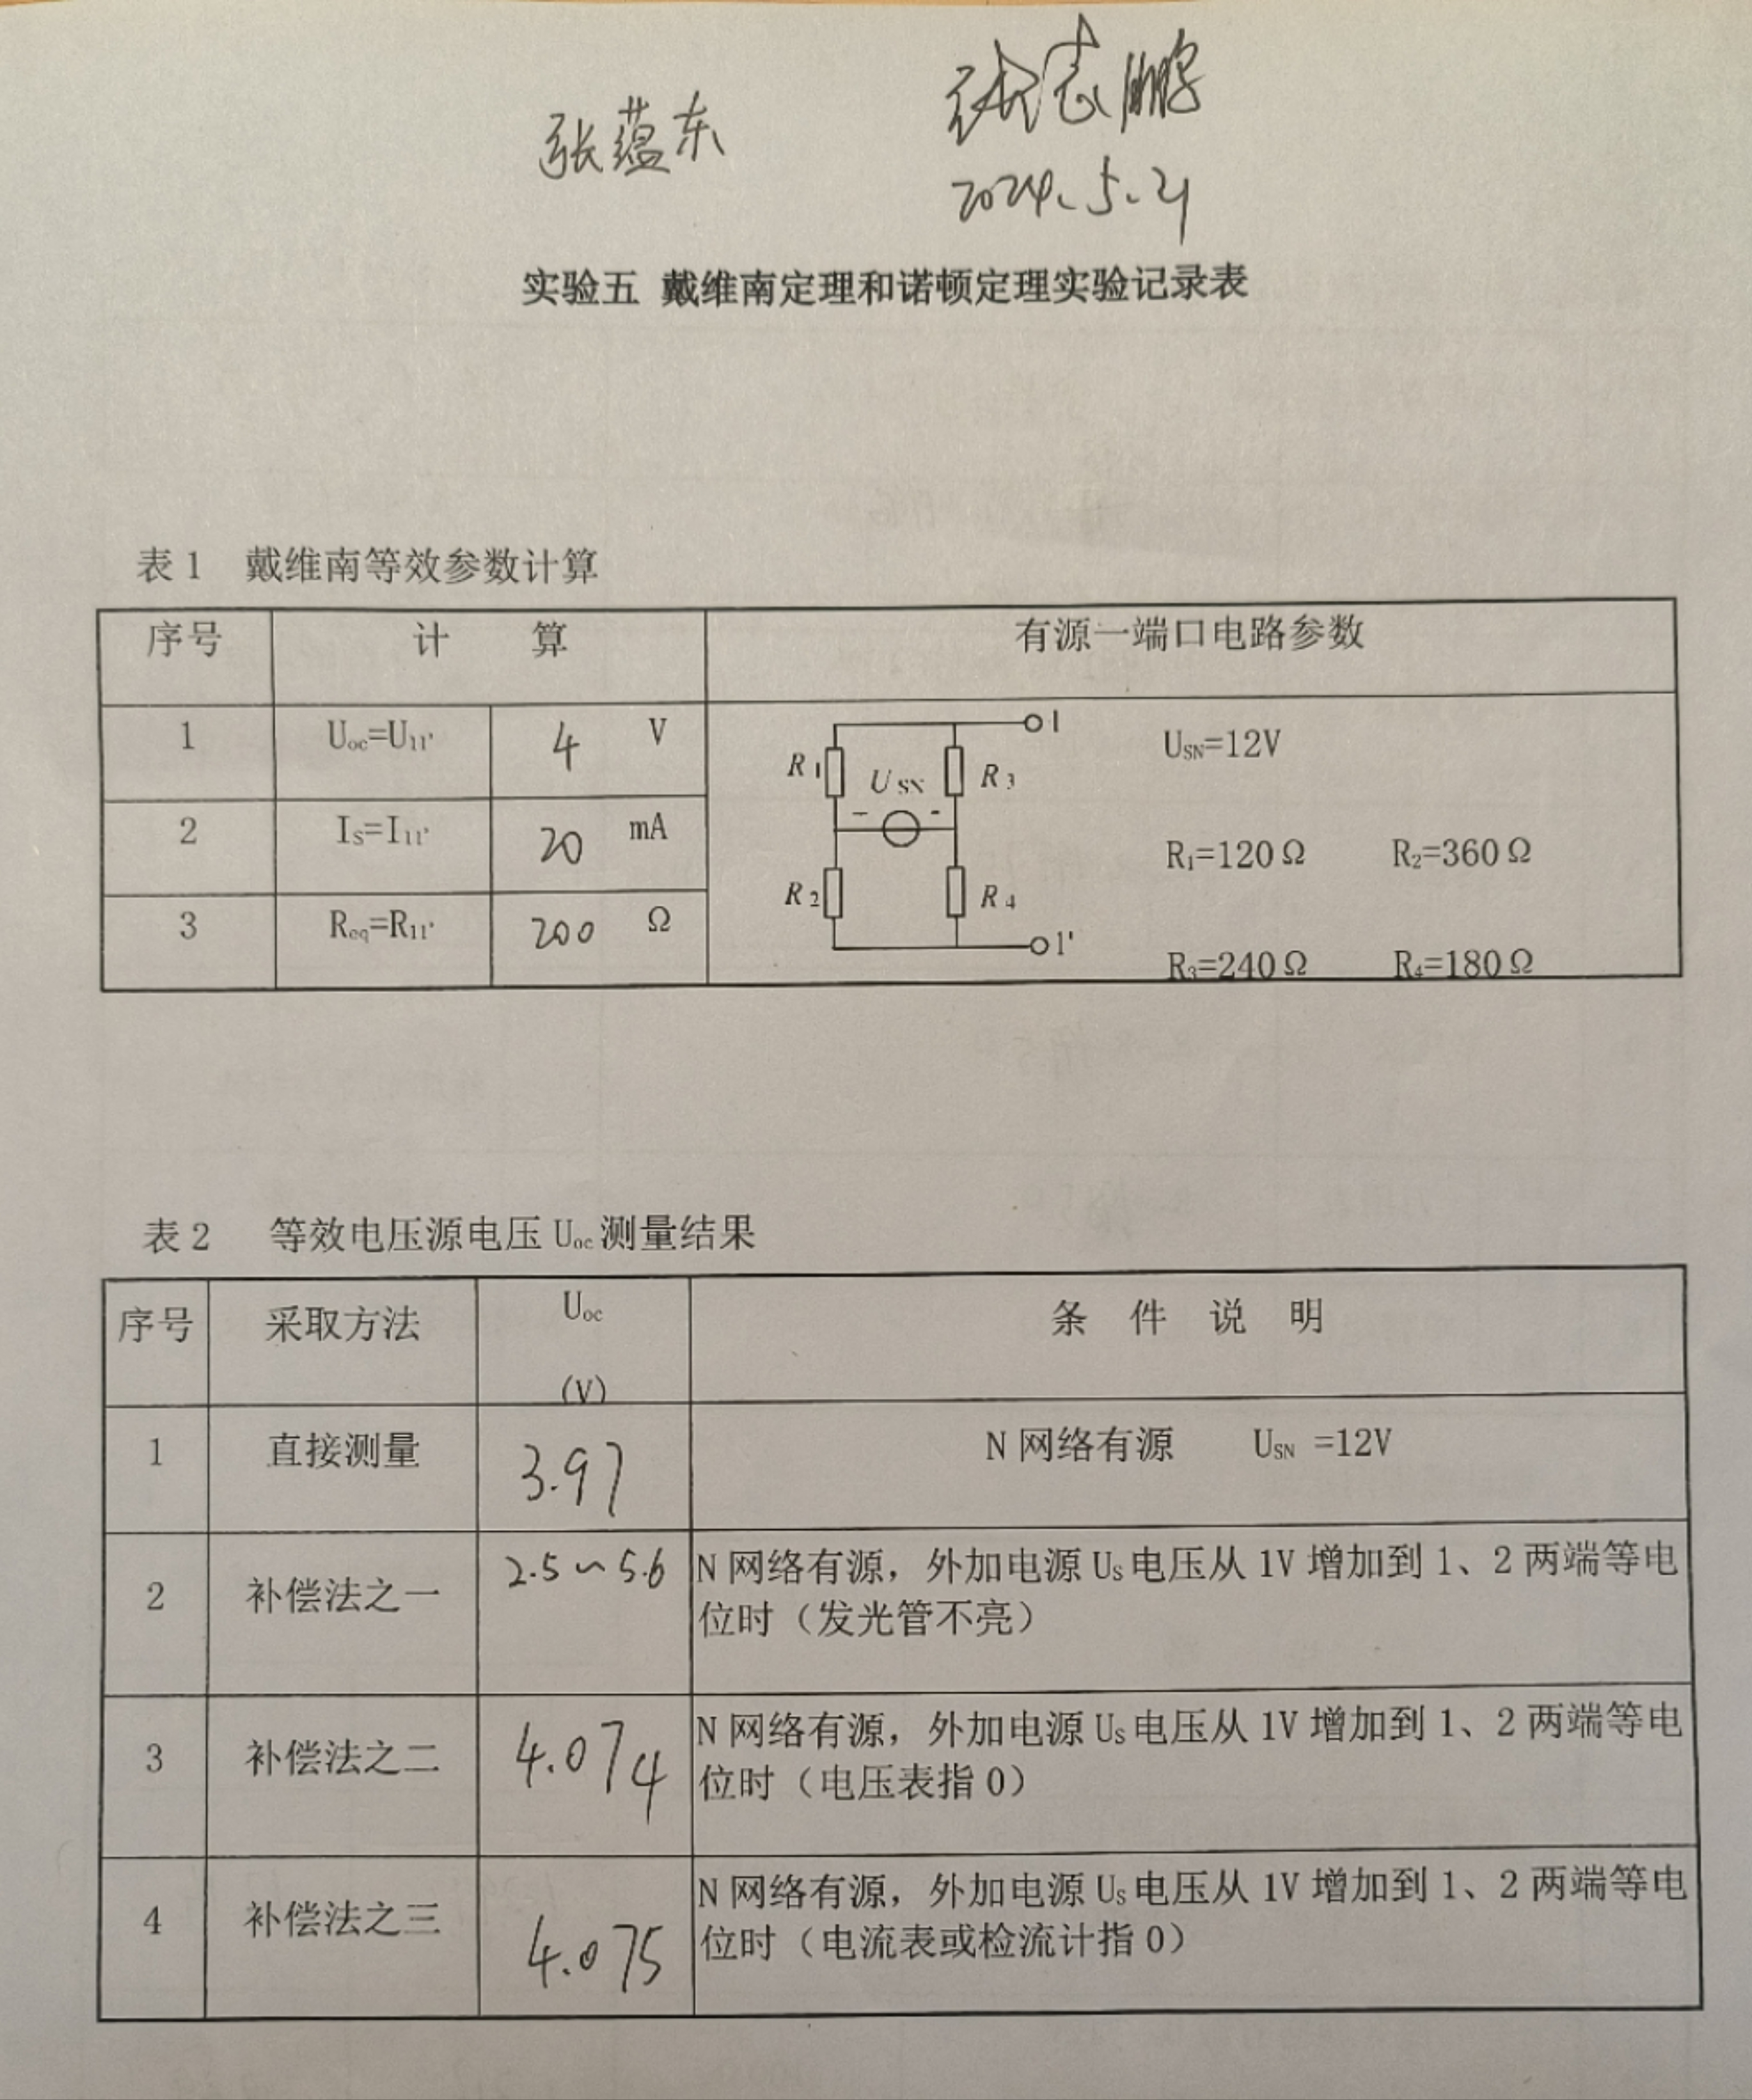
\includegraphics[width=0.95\textwidth]{2.jpg}}\newpage
    \framebox{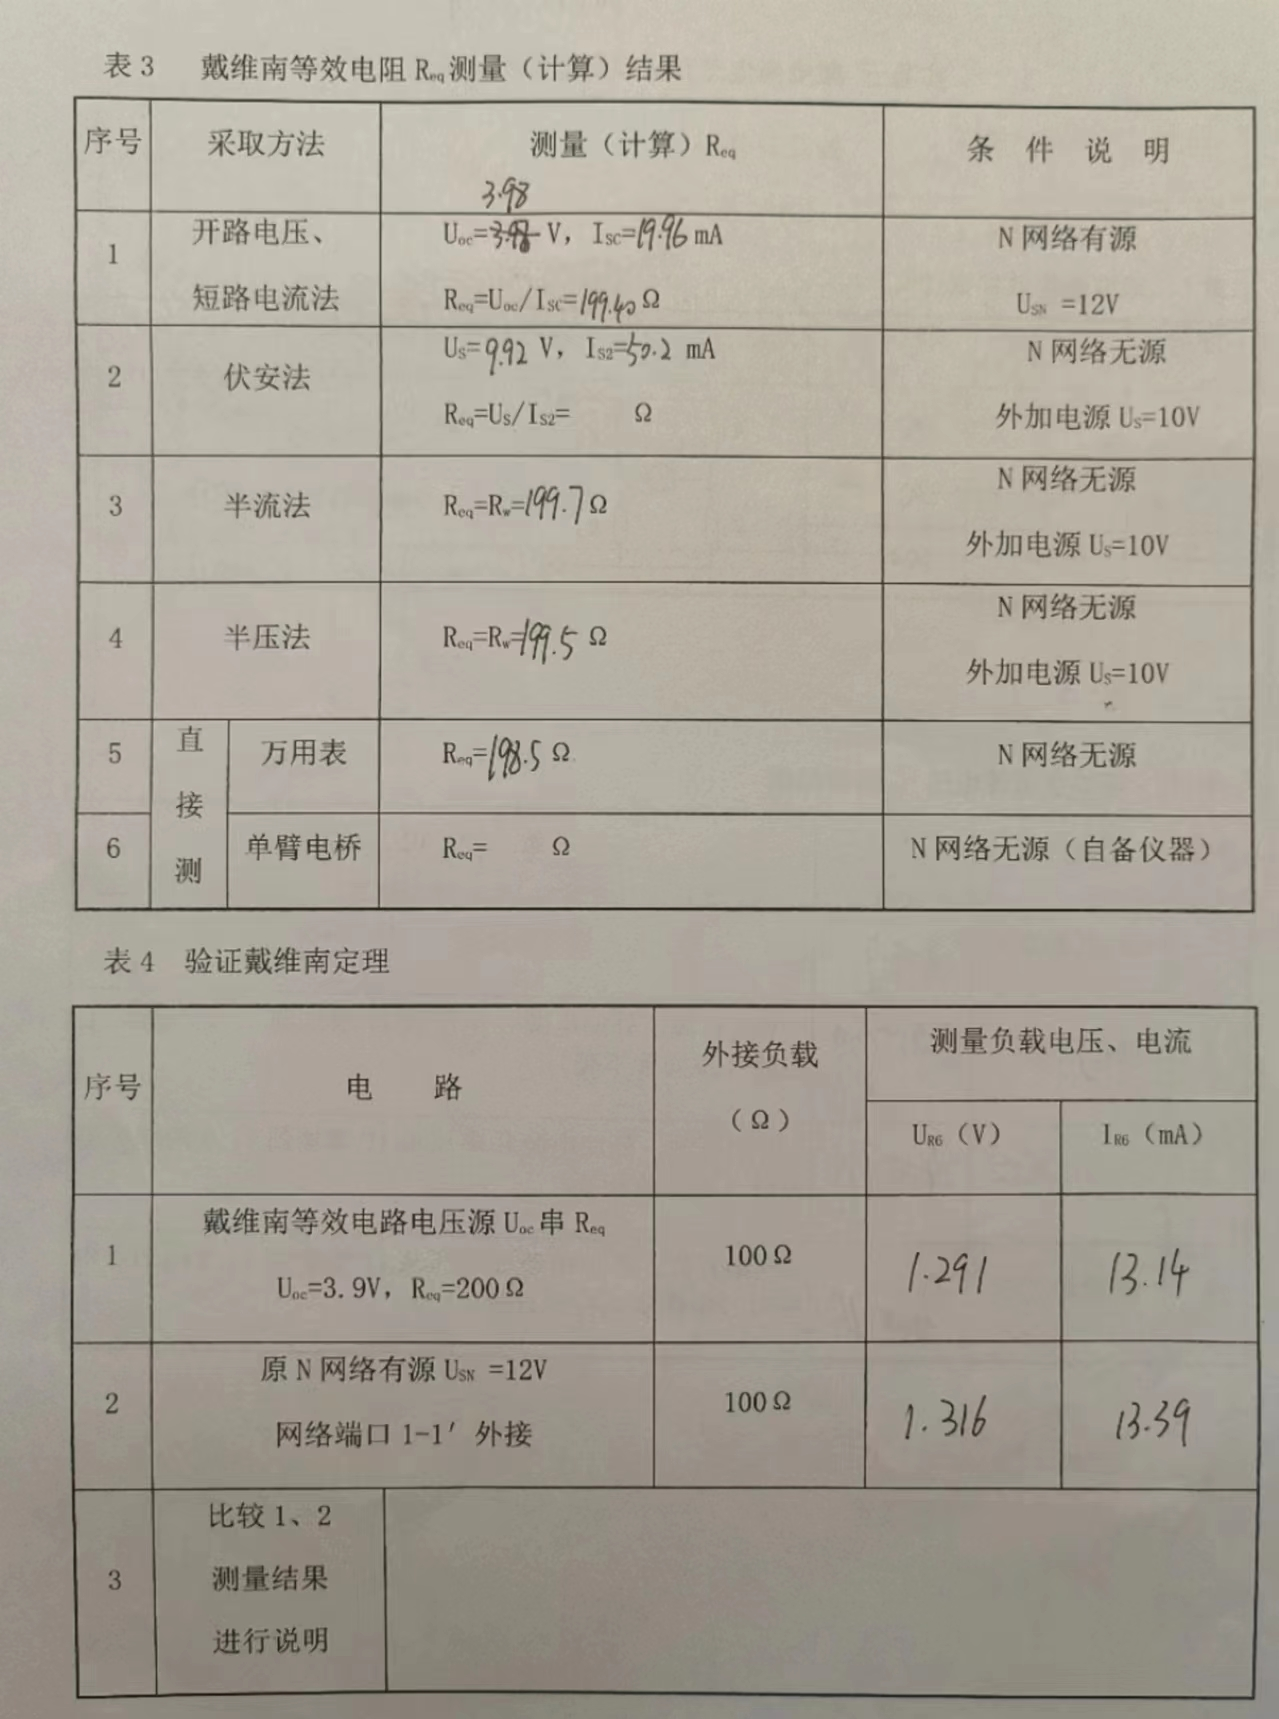
\includegraphics[width=0.95\textwidth]{3.jpg}}\newpage
    \framebox{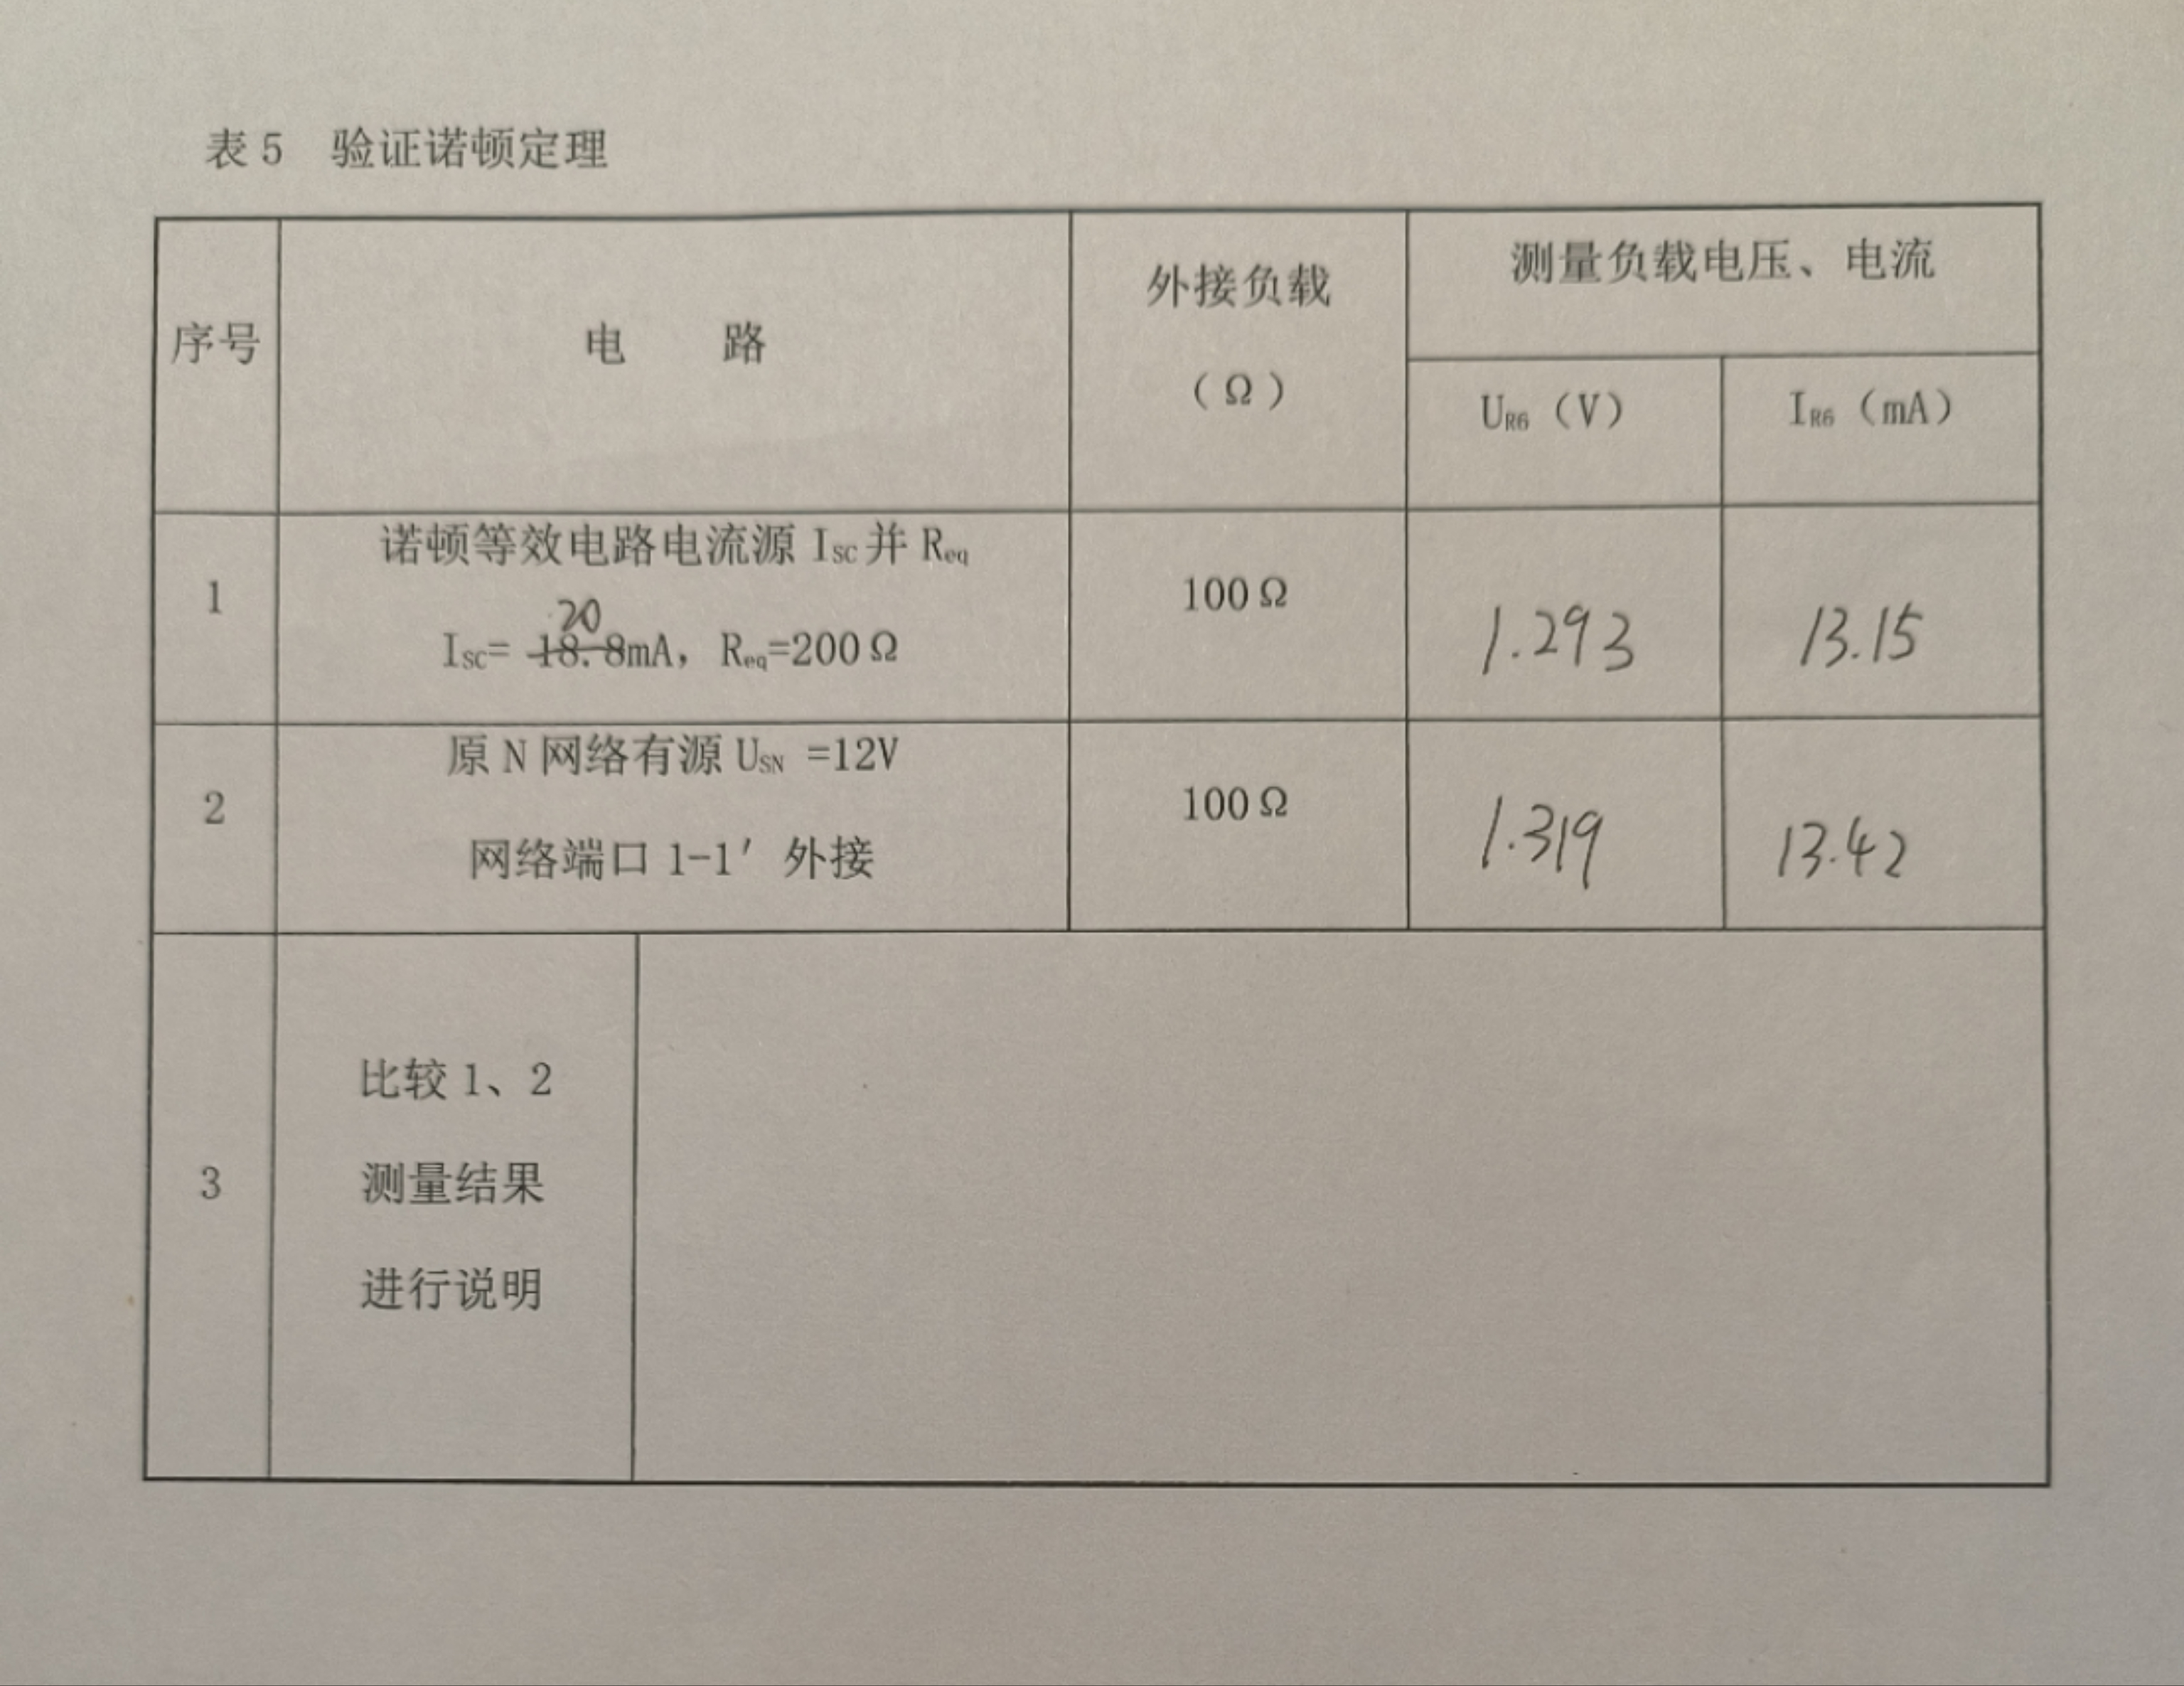
\includegraphics[width=0.95\textwidth]{4.jpg}}
\end{center}

\end{document}